\section{NoLin2Text}
% 我们的方法目的是帮助节点链接图的创作者自动生成辅助性语句,帮助节点链接图的目标观众理解节点链接图所要表达的内容。
We present \ApproachName~to generate presentation-aided statements automatically for node-link diagrams creators. The generated statements are aimed to facilitate the comprehension of the created node-link diagrams for target audiences.
% 为了生成能够帮助观众理解的语句,我们需要通过分析节点链接图的构建过程,来寻找观众会对节点链接图产生疑惑的原因。
To generate such presentation-aided statements, we need to decompose the creation process of node-link diagrams to explore the reasons for the audiences' confusion.
% 一个节点链接图的创作过程普遍会有以下X个步骤(其中第2步和第3步的顺序可以调换)[这里需要引一些文献]
% 1. 数据预处理;一般而言,真实世界收集到的源数据常常是表格型的多属性数据,而输入到节点链接图创作的图数据,往往是在源数据的基础上进行预处理,通过在源数据上定义实体之间的关系(链接),最终获得输入到节点链接图的图数据(包含节点和链接)
% 2. 设计可视编码;创作者还会把他想表达的数据特征编码到节点链接图上,比如利用节点的颜色来编码节点的类别等。
% 3. 计算图布局;节点链接图需要解决的一个关键问题是如何在二维空间中放置节点。链接则往往被绘制为节点之间的连接线,其位置往往由其两个端点决定。基于布局算法产生的节点位置,节点链接图才能进行绘制。
The creation of node-link diagrams commonly includes the following steps (the order of step 2 and step 3 can be reversed)~\cite{DBLP:journals/cgf/SpritzerBDFF15, tvcg/RomatAP21}:
\begin{compactenum}[\textbf{Step} 1.]
    \item \textbf{Graph wrangling}. Original data collected from the real world are rarely conforms to graph data, while node-link diagrams often employ data with specific and explicit nodes and links as input. They are usually wrangled from tabular data by defining relationships between entities~\cite{DBLP:journals/tvcg/SrinivasanPEB18, DBLP:conf/ieeevast/BigelowNML19, DBLP:journals/ivs/HeerP14, DBLP:journals/ivs/LiuNS14}.
    \item \textbf{Layout computing}. One key step of visualizing node-link diagrams is how to place nodes in a two-dimensional space. And links are placed according to two nodes each link connected.
    \item \textbf{Visual encoding}. To present data features of the underlying graph data, creators will encode several attributes they want to express with different visual channels. For example, the fill color of one node can be used to encode the category of it.
\end{compactenum}

% 我们提供了一个简单的usage scenario来展示该过程,从而导出我们的动机和解决方案。
% 我们主要聚焦于无向的同构图.
We present a simple usage scenario to demonstrate the process and then derivate our motivation and solutions.
In this paper, we focus on undirected homogeneous graphs.


\subsection{Usage Scenario and Motivations}

% 我们用 一个 imdb的电影数据集作为示例(https://www.kaggle.com/stefanoleone992/imdb-extensive-dataset)
% 为了表达 自2020年以来的电影之间是否存在相同的主演。我们将存在相同演员的电影用一条边进行链接,并且为这条边添加一个属性,叫做共享的相同的演员。
% 然后,我们用颜色来表示电影的出版月,用大小编码了它的预算(budget),用共享相同演员的数量来编码边的粗细。
% 最后,我们平均分编码节点横坐标,用评分人数编码纵坐标,生成一个节点链接图。
% 然而,上面的描述完全没有在节点链接图中体现,观众只能看到一些图形。
% 如果能够一些描述性的语句阐述其创作过程,作为可视化的辅助,那么观众就能对创作者的意图有所领悟。
% 我们的方法为它生成了以下的描述:
% ``节点之间因为 它们的actors属性拥有交集 而链接在一起。每个节点由一个circle组成。每条边由一个line组成。每个节点的circle的fill和它的date_published属性相关,r和它的budget属性相关,cx和它的avg_vote相关,cy和votes相关。每个链接的line的stroke-width和它的shared actors相关。''
We employ the IMDb movies dataset\footnote{https://www.kaggle.com/stefanoleone992/imdb-extensive-dataset} to create a node-link diagram as a demonstration to show the creation process.

\textbf{Data wrangling}. 
We select movies published in 2019 and show whether they share same actors.
Thus, we connect two movies with a link if the intersection of two movies' ``actors'' attribute are not null.
We also create an attribute for the link named ``shared\_actors'' to store the intersection.

\textbf{Visual encoding}.
After creating the graph data, we begin to program a node-link diagram to visualize the graph data.
Movies are encoded as circles with their color showing the ``published\_data'' attribute and radius showing the ``budget'' attribute.
We also encode the size of ``shared\_actors'' as the thickness of links.

\textbf{Layout computing}.
At last, we specific the layout. We do not choose any topology-based algorithm to generate the layout. 
Whereas, we encode the attributes ``ave\_vote'' and ``votes'' with the two-dimension position.

With such a node-link diagram, audiences can not obtain any information with only several graphics (Figure~\ref{fig:IMDbDiagram} (a)).
If several statements about the creation process can be presented to aid the visualization, audiences can reach a higher cognition.
Our approach generate such description for it:
\begin{lightgrayleftbar}\noindent
    Nodes are connected because there is an intersection between their ``actors'' attributes.
    Each node consists of a circle and each link consists of a line.
    The ``fill'' (color) of the circle corresponds to the node's ``date\_published'' attributes and the ``r'' (radius) of the circle corresponds to ``budget'' attributes.
    The ``stroke-width'' of the line corresponds to the link's ``shared\_actors'' attributes.
    The layout is attribtue-based.
    The abscissa of a node corresponds the node's ``ave\_vote'' attribute.
    The ordinate of a node corresponds the node's ``votes'' attribute.
\end{lightgrayleftbar}

\begin{figure}
    \centering
    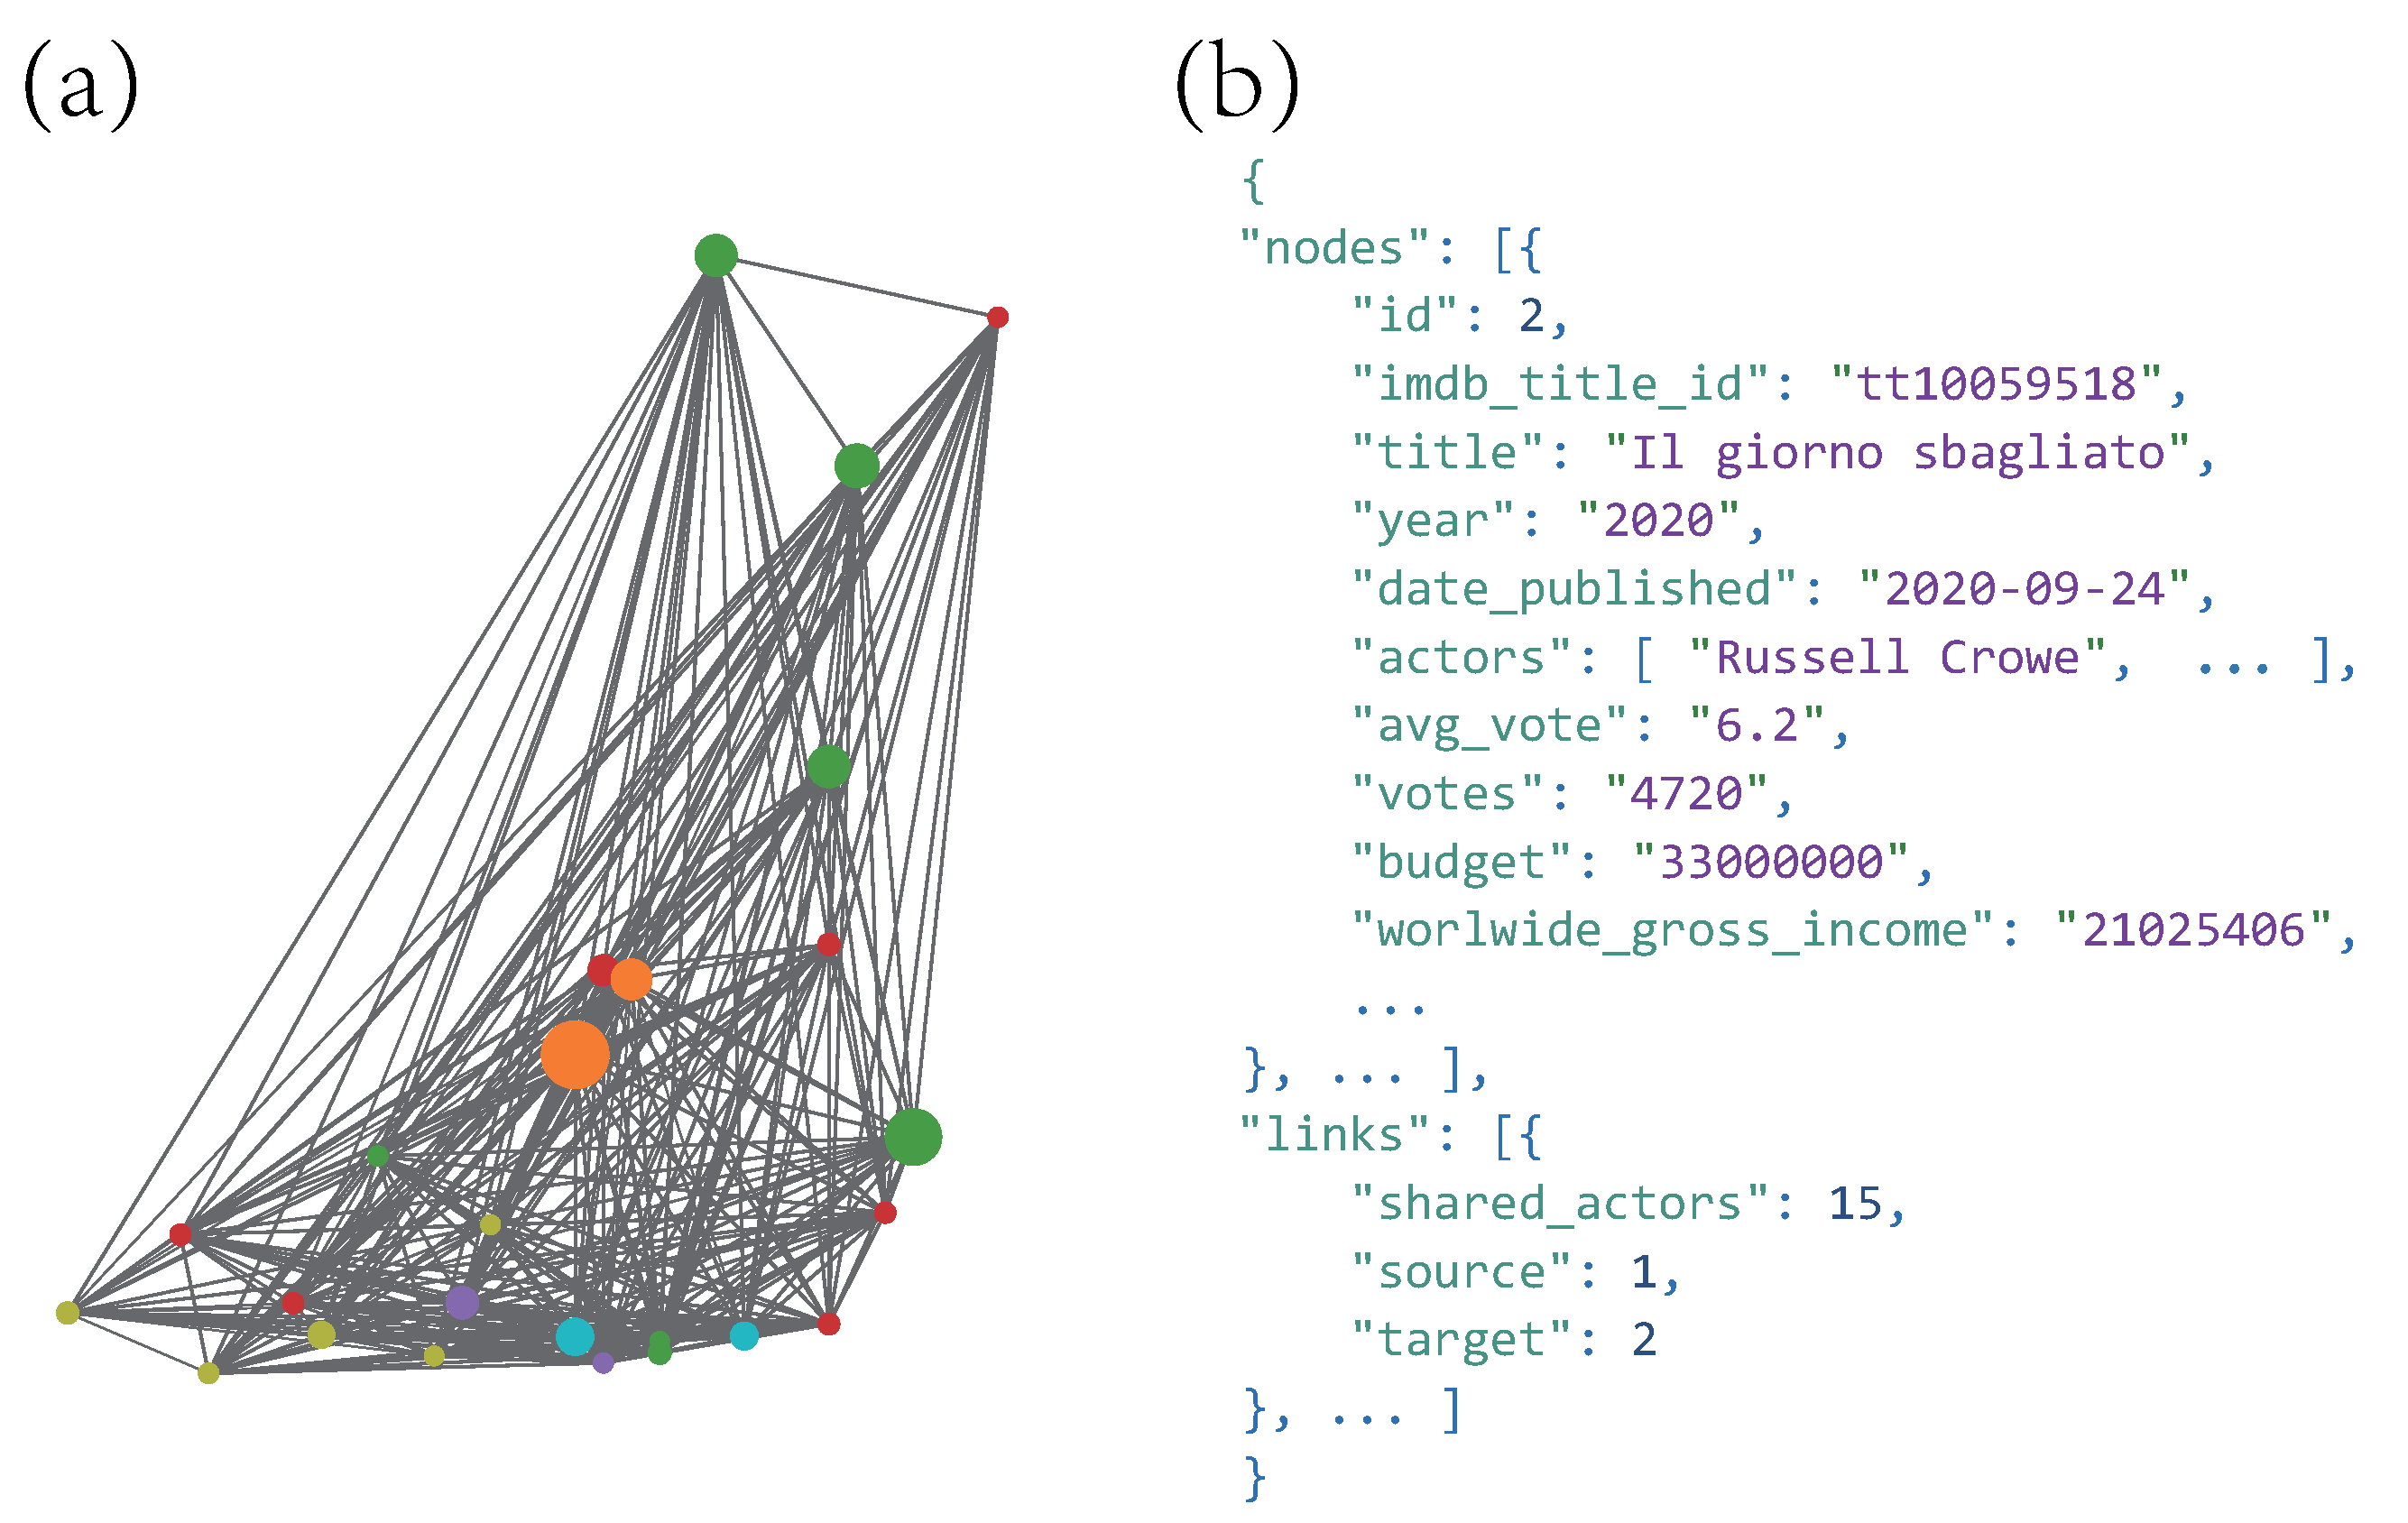
\includegraphics[width=1\columnwidth]{firgures/IMDbDiagram}
    \caption{ (a) A node-link diagram shows whether movies published in 2019 and whether they share same actors. (b) The underlying node-link formatted graph data.}
    \label{fig:IMDbDiagram}
\end{figure}

% 通过这个场景,我们看到了生成文本来提升节点链接图可理解性的必要性。
% 节点链接图的创作者有必要向其观众解释数据的生成、节点的编码、布局的目的等等。
% 相比于创造,编写解释性的文本往往枯燥乏味,因为该过程没有新的知识产生,仅仅是复述创作代码的历程而已。
% 一个有趣的例子是很多程序员对于编写注释往往比较抗拒。
% 于是,我们的方法想将这个过程自动化,以消除该繁琐的过程。
% 因为创作者已经将他的想法注入到代码中,我们只需要分析他的源码和输入的数据,进而就能够从中提取信息,然后将信息注入模板中生成描述。
From this scenario, it is obviously that presentation-aided statements are crutial for improving the comprehensibility of node-link diagrams.
It is necessary for creators to explain how the graph data is generated, how the attributes are encoded with visual channels, what the layout means, and so on.
Compared to creating the diagram, it is tedious to describe it, because nothing new is generated during describing.
It is just a retelling of the process of creating the diagram.
We aim to eliminate such a repeative process by automatically generating a serials of presentation-aided statements.
Because creators have injected his creation intention into the code, we only need to analyze the code and the input graph data to obtain the information. And at last we employ the obtained information to generate a template-based statements.

% 下面三个章节将会进一步对创作过程进行分析,总结节点链接图能够展示和不能够展示的信息。
% 对于不能展示的信息,我们提出了一些抽取方式进行提取,并为他们提供了一个文本模板,以便向观众介绍。
In following three subsections, we will futher discuss the creation process and summarize the information that node-link diagrams are able or unable to convey.
We propose several methods to extract the uncommitted information and provide corresponding textual templates to inform audiences.

% % 我们通过分析节点链接图创建过程中被隐藏的信息,用文本的形式显式揭露这些用户未知的信息,达到帮助理解的目的。
% % From this scenario, we propose three aspects to understand the diagram in light of the three-step creation process:
% % \begin{compactenum}
% %     \item \textbf{Understanding relationship} by revealing why nodes are connected.
% %     \item \textbf{Understanding encodings} by revealing how visual channels encode data attributes.
% %     \item \textbf{Understanding layout} by revealing what the layout encodes.
% % \end{compactenum}
% % 我们的方法采用图数据和创作者的节点链接图创作代码作为输入,最后输出关于这四个understanding的辅助性解释文本。
% % Our approach employ the node-link formatted graph data (Figure~\ref{fig:IMDbDiagram}(b)) and the code creating the diagram as input, and outputs a template-based textual statements to solve the three-undestandings.

\subsection{Data wrangling}
% 从表格型数据创建图数据时,最重要的就是建立节点之间的关系。
% 观众从节点链接图中所能获知的信息仅仅是某两个节点之间存在联系,但却不了解联系的内在含义。
% 一些论文已经对可能建立链接的情况进行了定义,
Several works~\cite{DBLP:journals/ivs/LiuNS14, DBLP:journals/ivs/HeerP14, DBLP:journals/tvcg/SrinivasanPEB18} about graph wrangling identify link construction as the crutial process.
Audiences can only obtain that two nodes are connected by a link by observing the diagram, while they do not know why nodes are connected.
Works mentioned above have proposed several conditions.
Ploceus~\cite{DBLP:journals/ivs/LiuNS14} and Orion~\cite{DBLP:journals/ivs/HeerP14} infer potential linking conditions by first constructing a linking graph and then searching valid linking paths. They are aimed at constructing links among multiple data tables by analyzing primary keys and foreign keys.
Graphiti~\cite{DBLP:journals/tvcg/SrinivasanPEB18} identifies potential linking conditions of a homogeneous graph by comparing different attributes.
% 如果多个表合并成一个表,前两者总结的条件可以被Graphiti提出的规则所覆盖
Because multiple tables can be merged into one data table with primary keys and foreign keys, Graphiti can cover the linking conditions identifying rules proposed by Ploceus and Orion. %? 这里mayby要用一张图解释一下
Three conditions are proposed by Graphiti:

\begin{compactenum}[\textbf{Condition} 1.]
    \item Sharing the same value of a categorical attribute between two nodes, e.g., linking two movies with a same director.
    \item Sharing the same common values or topics of a list or textual attribute between two nodes, e.g., linking two movies with one or more same actors. 
    \item Sharing the same, significantly close, or values in the same bin between two nodes, e.g., linking two movies if they are published within one week.
\end{compactenum}

% 我们尝试从它们的反方向进行思考,也就是,当我们获取到了所有的链接的时候,推测这些链接是如何被构建的
Those works infer the potential linking conditions before all links are constructed. 
Whereas, our method runs in the opposite direction where all links have been constructed already.
% ? 这里可能有多个条件的组合问题,有待进一步了解

\subsection{Understanding Visual Encodings}
%! 首先说明目标是什么
% 为了能够向观众解释节点链接图的编码是什么,我们希望通过分析创作者使用的图数据,创作者编写的代码,得到他使用的编码方案。我们通过三个层次来叙述节点链接图的编码方案:
% 1. 节点/链接的组成元素分别是什么?
% 2. 视觉通道的决定性因素(属性)是什么?
% 3. 视觉通道和其决定性因素的相关性如何?(正相关/负相关/类别相关..)


%! Deconstructing and Restyling D3 Visualizations 的一些不足之处
%! 1. __data__的依赖
%! 2. 映射关系的检验
%TODO: 可能还存在一些不足,在实现的时候可以被发现
% Deconstructing and Restyling D3 Visualizations 对于解决上述问题提出了一些很有见解的解决方法。但它也有一些不足之处。
% 1. 其需要创作者使用d3的数据绑定,才能发挥__data__的作用;使用其他工具,或者未将数据绑定到元素上时则无法使用该方法;
% 2. 其检验视觉通道和属性之间的关联,是通过检验属性和视觉通道之间是否存在线性映射或者类别性映射。在以下两种情况下该方法会失效:
%   2.1 如果不同的数据属性之间相互是线性相关的,那么该方法就无法真正确定是哪一种属性决定了视觉通道;
%   2.2 其检验的映射过于简单,复杂情形下无法得到相互关联的结论;

% 我们尝试从这几个方向增强该方法,并配合节点链接图的特性,帮助创作者更好的解释节点链接图中的编码方案。
% 我们发现,虽然 Deconstructing and Restyling D3 Visualizations 的方法只需要svg作为方法的输入,但它的svg是处于运行环境中的,也就是说,如果没有运行源代码,__data__属性也就没法绑定到对应的元素中。所以它隐式地依赖于可视化创作者的源代码。所以我们还可以使用其源代码用于分析。


%! 我们的方法的过程
% 我们对Deconstructing and Restyling D3 Visualizations进行了改进;主要从x方面进行:
% 作为该方法的补充,为了使数据绑定能够应用于非d3创建的代码,我们提出了一个检验方法,它将创建者创建的代码视作黑盒,通过修改输入的数据,检验输出的svg元素的变化来获取编码方案。
%? 这里假设了修改源数据,不会对代码造成影响,但实际上很多情况下,映射方式会根据数据本身进行更改,比如数据值的范围。可以放在discussion里面讨论一下。
% 下面的章节我们围绕着几个方面进行:
% 1. 如何为没有为没有进行数据绑定的svg,找到每个节点和链接对应的元素,以补充 Deconstructing and Restyling D3 Visualizations;
% 2. 新的视觉通道和属性之间的关联检验方式,防止出现多属性之间线性依赖以及复杂映射情形失效的情况;
% TODO下面都是围绕节点和链接展开,但我们的方法不仅仅能够解决节点链接图的可视化,也可以用用于其他类型的可视化形式。

%! 讲一下我们主要检测的基础视觉元素:

%! 1 首先对某个属性做出修改,但不修改数据分布,只调换数据顺序;查看哪个/些视觉通道发生了变化;找到那些不改变dom结构的属性(tagname和element数量);
%!  对嵌套结构(数组/对象)进行说明:没有关系,等详细说明映射方式的时候再决定;
%! 2 过滤掉会对svg element的tagName和数量产生影响的属性,交换A节点和B节点的其余数据,观察哪些svg的视觉通道发生了变化;然后恢复数据;再交换A节点和C节点的其余数据,观察通道变化;取两次的交集的svg element,它们绑定的数据就是A节点;

\subsection{Understanding Layout}

\subsection{Interview \& Iterative Design}

\subsection{Understanding Visual Clutter}